\documentclass[conference,a4paper]{IEEEtran}
\IEEEoverridecommandlockouts
% Camera-ready version after double-blind review. Structured in IMRaD format.

\usepackage[nocompress]{cite}   % keeps citations separate and ordered: [1], [2], [3]
\usepackage{amsmath,amssymb,amsfonts}
\usepackage{graphicx}
\usepackage{textcomp}
\usepackage{xcolor}
\usepackage{booktabs}
\usepackage{multirow}

% --- Margin compliance -------------------------------------------------------
% IEEEtran's default text block starts ~0.68 in from the top of US Letter, below the
% 0.75 in the submission system requires. Shift the block down and shorten it by the
% same amount so the bottom margin is preserved.
\addtolength{\topmargin}{0.15in}
\addtolength{\textheight}{-0.15in}
% -----------------------------------------------------------------------------

\newcommand{\pr}{\mathbf{p}}
\newcommand{\rc}{SA\mbox{-}WSV}
\newcommand{\rcz}{SA\mbox{-}WSV$_0$}
\newcommand{\rco}{SA\mbox{-}WSV$_1$}

\begin{document}

\pdfinfo{
/Title (Shrinkage-Adaptive Weighted Soft Voting for Ensembles of Indonesian Pre-Trained Language Models in Electric Vehicle Sentiment Classification)
/Author (Budi Juarto; Kania Alma Tiara)
/Keywords (sentiment analysis; electric vehicles; Indonesian; pre-trained language models; ensemble learning; James-Stein shrinkage; calibration; risk control)
}

\title{Shrinkage-Adaptive Weighted Soft Voting for Ensembles of Indonesian Pre-Trained Language Models in Electric Vehicle Sentiment Classification}

\author{
\IEEEauthorblockN{1\textsuperscript{st} Budi Juarto\textsuperscript{*}}
\IEEEauthorblockA{\textit{Computer Science Department}\\
\textit{Bina Nusantara University}\\
Jakarta, Indonesia\\
budi.juarto@binus.ac.id}
\and
\IEEEauthorblockN{2\textsuperscript{nd} Kania Alma Tiara}
\IEEEauthorblockA{\textit{Creativepreneurship Program}\\
\textit{Bina Nusantara University}\\
Jakarta, Indonesia\\
kania.tiara@binus.ac.id}
}

% Recover part of the space added by the author block.
\IEEEaftertitletext{\vspace{-1.5\baselineskip}}
\maketitle

\begin{abstract}
Ensembles of pre-trained language models (PLMs) are a common remedy for short, colloquial texts such as Indonesian electric vehicle (EV) posts, but their fusion rules are rarely compared under identical conditions. We fine-tune five Indonesian and multilingual PLMs on three EV sentiment corpora with 5-fold cross-validation and five seeds (375 runs) and score 26 fusion rules on the same posteriors. Encoder choice dominates: monolingual encoders beat multilingual BERT by 3.5 to 7.9 macro-F1 points. With the encoders fixed, no rule, stacking included, beats uniform soft voting after multiplicity correction, because the learners err together (2.1 to 2.4 effective independent voters of five). We propose shrinkage-adaptive weighted soft voting (\rc), which shrinks validation reliabilities toward equality by a James--Stein factor with a paired-bootstrap noise term; the bootstrap confirms each learner's binomial macro-F1 variance but shows that ignoring the shared validation split overstates the noise in learner differences 2.2-fold. \rc{} is a risk-control rule, not an accuracy booster: over 900 small-validation deployments its confidence-free form never loses more than 0.5 points to uniform voting (worst-5\% mean \textminus0.25), against \textminus2.2 to \textminus2.6 for learned weights, and it neutralises a corrupted learner that costs uniform voting 0.55 points. An instance-level confidence term raises the mean slightly but enlarges the tail, as the learners are over-confident on different scales. Zero-shot transfer between corpora costs up to 31 points, and posts missed by every model were mostly revised by the second annotator.
\end{abstract}

\begin{IEEEkeywords}
sentiment analysis, electric vehicles, Indonesian pre-trained language models, ensemble learning, James--Stein shrinkage
\end{IEEEkeywords}

\section{Introduction}

Indonesia has made electric vehicles (EVs) a policy priority, and the debate about prices, subsidies, battery durability and charging is widely voiced on social media \cite{saraswati2025}, which makes EV sentiment analysis an active application area \cite{ekatama2023, saraswati2025}. The posts are short, informal, code-mixed and full of non-standard spellings. PLMs \cite{devlin2019} adapted to Indonesian \cite{wilie2020} are the usual remedy, and because labelled EV corpora are small, several are often combined into an ensemble \cite{ganaie2022}. Many weighting recipes exist, but each paper uses its own corpora, splits and learners, so a reported gain cannot be attributed to the weighting rule; with one fine-tuning seed per learner, part of any difference is seed noise \cite{bouthillier2021, sellam2022}.

\subsection{Related Work}

\textbf{EV opinion mining.} Transformers have classified 127k EV charging-station reviews \cite{ha2021}. Indonesian EV studies often use support vector machines \cite{alhari2022, ekatama2023, saraswati2025}; IndoBERT beat a FastText baseline on EV tweets \cite{wijaya2024}, and recent work uses IndoBERT and DeBERTa for policy comments \cite{nugroho2025}, IndoBERT and IndoRoBERTa for aspect-based analysis \cite{canavara2025}, and zero-shot inference pipelines on multilingual XLM-RoBERTa \cite{nugroho2024zero}. Multilingual encoders such as XLM-R \cite{conneau2020} transfer across languages, but tokenizer quality and pre-training data explain much of their gap to monolingual models \cite{rust2021}.

\textbf{Ensembles of neural text classifiers.} Weighted and majority voting of fine-tuned transformers with weights proportional to each model's accuracy improved Bangla sentiment \cite{seth2023}; confidence-weighted voting was applied to software engineering sentiment \cite{batra2021}; dynamic uncertainty weighting combines heterogeneous learners \cite{yang2025}; and weighted averaging of a Transformer and an FNet has used their mean late-epoch validation accuracies as weights \cite{wu2026}. Elgabry and Hamdi weight each model's class probabilities by its validation macro-F1 \cite{elgabry2026}, which is linear-F1 weighting below. For Indonesian hate speech, equal-weight soft voting of IndoBERTweet and IndoRoBERTa matched its stronger member and was better calibrated \cite{alkaff2026}. Learned combiners such as stacking are standard \cite{ganaie2022}, but optimised weights can overfit limited validation data \cite{purucker2023}.

\textbf{Reliability, calibration and annotation.} For conditionally independent voters the optimal weighted majority uses log-odds weights \cite{kuncheva2014}; shrinking noisy estimates toward a common mean is the classical remedy when data are scarce \cite{efron2021}. Neural posteriors are miscalibrated, and temperature scaling is the standard fix, also for PLMs \cite{guo2017, xiao2022}. Disagreement between out-of-sample predictions and the gold label detects annotation errors \cite{klie2023, northcutt2021}, though part of it reflects genuine label variation \cite{plank2022}.

\subsection{Contributions}
(i) Five PLMs are fine-tuned on three EV corpora with 5-fold cross-validation and five seeds, and 26 fusion rules, including recent and learned baselines, are scored on identical posteriors with a two-stage bootstrap over seeds and test instances. (ii) We measure why the rule barely matters: errors are strongly correlated, and a paired bootstrap shows how well a validation split ranks learners. (iii) We propose \rc, which shrinks reliability estimates by a James--Stein factor estimated from that bootstrap, and evaluate it as risk control: tail risk over small-validation deployments, a corrupted-learner stress test, and its confidence term and calibration. (iv) Transfer in ten directions and an annotation analysis show where the remaining errors lie.

\section{Method}
\label{sec:method}

\subsection{Weighted Soft Voting}
Let $\mathcal{D}=\{(x_i,y_i)\}_{i=1}^{N}$ be texts with labels $y_i\in\{1,\dots,C\}$, here $C=2$. Learner $m\in\{1,\dots,M\}$ is a PLM encoder $g_m$ with a linear head, $\pr_m(x)=\mathrm{softmax}(W_m g_m(x)+b_m)$, fine-tuned with cross-entropy. A weighted soft-voting ensemble predicts
\begin{equation}
\hat{y}=\arg\max_{y}\sum_{m=1}^{M}\omega_m(x)\,p_m(y\mid x),\qquad \textstyle\sum_{m}\omega_m(x)=1,
\label{eq:wsv}
\end{equation}
which is uniform soft voting when $\omega_m=1/M$. The rules compared differ only in $\omega_m(x)$.

\subsection{Reliability and Confidence Terms}
For $M$ conditionally independent voters with accuracies $a_m>1/2$, the optimal weighted majority weights voter $m$ by $\ln(a_m/(1-a_m))$ \cite{kuncheva2014}. \rc{} borrows this form as a heuristic, not as a consequence of that result, with the validation macro-F1 $F_m$ in place of accuracy:
\begin{equation}
w(F)=\ln\frac{F}{1-F},\qquad F\leftarrow\min\big(\max(F,\tfrac12+\epsilon),1-\epsilon\big),
\label{eq:reliability}
\end{equation}
with $\epsilon=10^{-6}$, so a learner no better than chance gets practically no weight. Both departures from the theorem are measured rather than assumed: on these binary, near-balanced corpora validation macro-F1 and accuracy differ by at most 0.006, changing the normalised weights by at most 0.003, whereas the independence assumption fails clearly (Section~\ref{sec:noise}). The instance-level term is the normalised entropy $c_m(x)=1-H(\pr_m(x))/\ln C\in[0,1]$.

\subsection{Shrinkage-Adaptive Weighting}
The weight $w(F_m)$ is only as good as $F_m$, which is estimated on 111 to 288 validation items. \rc{} therefore shrinks the estimates toward their mean, $\tilde F_m=\bar F+\lambda(F_m-\bar F)$, with the positive-part James--Stein factor \cite{efron2021}
\begin{equation}
\lambda=\max\Big(0,\;1-\frac{M-3}{M-1}\cdot\frac{\hat\tau^{2}}{\lVert\mathbf d\rVert^{2}}\Big),\qquad \mathbf d=\mathbf F-\bar F\mathbf 1,
\label{eq:lambda}
\end{equation}
where $\hat\tau^2$ estimates $\mathrm{E}\lVert\mathbf d\rVert^2$ when all learners are equally reliable. The binomial value $\hat\tau^2=\frac{M-1}{Mn}\sum_m F_m(1-F_m)$ ignores the non-linearity of macro-F1 and the dependence between learners scored on the same items, so \rc{} uses a paired bootstrap: the validation split is resampled $B=1{,}000$ times with the same indices for every learner and $\hat\tau^2=\sum_m\widehat{\mathrm{Var}}_b(F^{(b)}_m-\bar F^{(b)})$. For independent learners with common variance $\sigma^2$, $\hat\tau^2=(M-1)\sigma^2$ and (\ref{eq:lambda}) is the classical factor $1-(M-3)\sigma^2/\lVert\mathbf d\rVert^2$. The weights are
\begin{equation}
\omega_m(x)=\frac{w(\tilde F_m)\,c_m(x)^{\gamma}}{\sum_{k}w(\tilde F_k)\,c_k(x)^{\gamma}},\qquad\gamma\in\{0,1\}.
\label{eq:omega}
\end{equation}
With $\gamma=0$ (\rcz) the rule is uniform soft voting when $\lambda=0$ and log-odds weighting when $\lambda=1$; with $\gamma=1$ (\rco) the $\lambda=0$ limit is entropy-confidence weighting. We also evaluate the binomial factor, a marginal bootstrap that keeps the independence assumption, a normal--normal empirical-Bayes estimator \cite{efron2021} with learner-specific variances, and bootstrap-averaged (bagged) weights.

\subsection{Corpora and Labelling Protocol}
\textbf{EV-Norm} and \textbf{EV-Raw} are two renderings of the same 1{,}382 Indonesian social media posts about EVs (691 negative, 691 positive, 25 words on average). Each post was labelled by one annotator and reviewed by a second, who confirmed or changed the label; the reviewed label is used throughout and the first-pass label is kept for the error analysis. EV-Raw keeps the colloquial text; for EV-Norm the annotators rewrote each post manually in standard Indonesian, resolving the slang, abbreviations and non-standard spellings typical of colloquial Indonesian \cite{wibowo2021}. \textbf{EV-Public} holds 3{,}592 public tweets and YouTube comments on EVs (April 2021 to May 2023; 1{,}620 negative) with an undocumented labelling protocol. Two public corpora serve only as transfer targets: \textbf{EV-Twitter}, 2{,}446 positive or negative tweets (September 2022 to February 2023) after removing duplicates and 26 texts shared with EV-Public, and \textbf{EV-YouTube}, 1{,}371 comments on the EV purchase incentive (September 2022 to August 2023), released lower-cased and stemmed. No other text is shared between corpora.

\subsection{Learners and Training Protocol}
The pool holds three monolingual Indonesian encoders, IndoBERT-p1 \cite{wilie2020} and the IndoBERT-1.5G and IndoRoBERTa-1.5G checkpoints trained on a 1.5\,GB Indonesian corpus, and two multilingual ones, XLM-R \cite{conneau2020} and multilingual BERT (mBERT) \cite{devlin2019}, with 110.6 to 278.0 million parameters. Each corpus is split by stratified 5-fold cross-validation, and a stratified 10\% of each training portion is the validation split that selects the checkpoint and fits every fusion rule; test portions are never used for fitting. Learners are fine-tuned for 3 epochs with AdamW (learning rate $2\times10^{-5}$, batch 16, weight decay 0.01, 10\% warm-up, clipping 1.0, 128 tokens), keeping the best validation checkpoint. Every configuration is trained with five seeds (42, 1 to 4), which change initialisation and data order \cite{sellam2022} and dropout \cite{bouthillier2021} while folds stay fixed: 375 runs on one RTX 3070 Ti Laptop GPU. Runs of seeds 1 to 4 also score, zero-shot, every corpus sharing no post with their training data.

\subsection{Fusion Rules Compared}
All 26 rules are fitted on the validation split only. (i) Twelve rules: the validation-selected single learner, majority voting, and ten soft-voting rules, namely uniform soft voting, linear-F1 weighting $\omega_m\propto F_m$ \cite{elgabry2026}, softmax-F1 weighting $\omega_m\propto e^{\beta F_m}$ ($\beta$ tuned on validation), log-odds weighting, max-probability and entropy confidence, three reliability--confidence products and the binomial \rco. (ii) Six further baselines: the product rule; late-epoch accuracy weights \cite{wu2026}; soft voting over temperature-scaled posteriors \cite{guo2017}; stacking with a cross-validated $L_2$-regularised logistic regression on validation logits; convex weights minimising validation log-loss; and greedy ensemble selection \cite{purucker2023}. (iii) Eight \rc{} variants: bootstrap \rco{} and \rcz, the alternative estimators and a covariance-aware factor, and \rco{} on temperature-scaled inputs or with percentile-normalised confidences.

\subsection{Evaluation and Statistical Analysis}
Following \cite{ulmer2022}, macro-F1 is averaged over folds and seeds. Each seed's predictions are pooled out of fold, and rule differences are tested with a two-stage bootstrap that resamples seeds and, jointly for all seeds, instances within folds ($B=5{,}000$), sharing resamples across rules so that comparisons are paired \cite{sellam2022}. We report percentile 95\% intervals and two-sided bootstrap $p$-values, Holm-corrected within each corpus over all 30 rules and learners; \rco{} against uniform voting was designated the primary comparison before the multi-seed runs and is also Holm-corrected over the three corpora alone. Rules are practically equivalent when the 90\% interval of their difference lies within $\pm0.5$ points, about a learner's seed-to-seed SD. Exact McNemar tests \cite{mcnemar1947} within each seed complement the bootstrap. Diversity is measured by the Q-statistic \cite{kuncheva2014} and the participation ratio of the error-correlation matrix (effective number of independent voters), calibration by expected calibration error (ECE, 15 bins) on pooled predictions. Risk is measured by refitting every rule on random validation subsets of 20, 40 and 80 items (20 draws per fold, all corpora and seeds; 900 deployments) and summarised by the mean difference to uniform voting, the mean of the worst 5\% (CVaR$_5$) and the share losing over 0.5 points, with intervals from a bootstrap over (corpus, seed) clusters. A stress test swaps one learner's class probabilities on a random fraction $\rho$ of validation and test items.

\section{Result}
\label{sec:result}

\subsection{Learners, Seeds and Calibration}
Table~\ref{tab:single} reports the learners. Every monolingual encoder beats mBERT on every corpus, by 3.5 to 7.9 points, significantly in all five seeds (exact McNemar, Holm). Against XLM-R the monolingual advantage is 2.6 to 4.4 points on EV-Norm and EV-Raw (significant in 23 of 30 seed-level tests), while on EV-Public XLM-R ties the IndoBERTs and leads IndoRoBERTa-1.5G by 1.5. Normalisation helps every learner, by 1.1 to 1.5 points and by 4.0 for mBERT. A learner's seed-to-seed SD is 0.27 to 1.27 points, as large as most differences between fusion rules. All learners are over-confident: the validation-fitted temperature exceeds 1 in 90\% of runs, learner-mean temperatures differ by a factor of 1.3 to 1.5 within a corpus (permutation $p<0.001$), and temperature scaling lowers pooled ECE by 48 to 66\% without changing any prediction.

\begin{table}[t]
\caption{Learners: macro-F1 (mean $\pm$ SD over five seeds of the 5-fold mean), validation-fitted temperature $T$ and pooled test ECE before/after temperature scaling (corpus average).}
\label{tab:single}
\centering
\footnotesize
\setlength{\tabcolsep}{2.2pt}
\begin{tabular}{lccccc}
\toprule
Learner & EV-Norm & EV-Public & EV-Raw & $T$ & ECE \\
\midrule
IndoBERT-p1      & 89.61$\pm$0.44 & 84.72$\pm$0.27 & 88.49$\pm$0.31 & 1.62 & .070/.030 \\
IndoBERT-1.5G    & 89.05$\pm$0.59 & 83.59$\pm$0.53 & 87.73$\pm$0.91 & 1.51 & .064/.025 \\
IndoRoBERTa-1.5G & 88.14$\pm$0.60 & 82.56$\pm$0.47 & 86.69$\pm$1.05 & 1.59 & .066/.029 \\
XLM-R            & 85.56$\pm$1.27 & 84.07$\pm$0.36 & 84.09$\pm$1.15 & 1.25 & .056/.026 \\
mBERT            & 84.65$\pm$1.10 & 78.60$\pm$0.41 & 80.62$\pm$0.72 & 1.32 & .062/.027 \\
\bottomrule
\end{tabular}
\end{table}

\subsection{Comparison of Fusion Rules}
Table~\ref{tab:fusion} reports the main rules. After Holm correction over the 30 rules and learners, only the validation-selected single learner differs from uniform soft voting, and it is worse (EV-Public). \rco{} gains $+0.06$, $+0.05$ and $+0.49$ points on EV-Norm, EV-Public and EV-Raw (95\% intervals $[-0.42, 0.51]$, $[-0.29, 0.39]$ and $[0.02, 0.97]$); the EV-Raw gain is not significant after Holm correction over the three corpora ($p=0.12$). \rcz{} stays within $[-0.20, 0.49]$ of uniform voting on every corpus. Eight of the nine other soft-voting rules of group (i) are practically equivalent to uniform voting within $\pm0.5$ points on EV-Norm and EV-Public, one on EV-Raw, and all nine within $\pm1$ point. With the full validation split the learned combiners have high means (stacking $+0.17$ to $+0.41$), with intervals that include zero. Within one seed the ten soft-voting rules of group (i) span up to 0.94 points, so single-seed comparisons exaggerate rule differences.

\begin{table}[t]
\caption{Macro-F1 of the main fusion rules (mean over five seeds of the 5-fold mean). $\dagger$: 95\% bootstrap interval of the difference to uniform soft voting excludes zero (uncorrected).}
\label{tab:fusion}
\centering
\footnotesize
\setlength{\tabcolsep}{3pt}
\begin{tabular}{lccc}
\toprule
Fusion rule & EV-Norm & EV-Public & EV-Raw \\
\midrule
Best single (val-selected)        & 88.91 & 84.25$^{\dagger}$ & 88.05 \\
Majority voting                   & 89.12 & 85.39 & 87.80$^{\dagger}$ \\
Uniform soft voting               & 89.27 & 85.50 & 88.24 \\
Linear-F1 weighting \cite{elgabry2026} & 89.25 & 85.51 & 88.32 \\
Softmax-F1 weighting              & 89.37 & 85.36 & 88.54 \\
Log-odds weighting                & 89.22 & 85.51 & 88.53 \\
Entropy confidence                & 89.30 & 85.53 & 88.56 \\
Log-odds $\times$ entropy         & 89.32 & 85.57 & 88.70 \\
Product rule                      & 89.25 & 85.56 & 88.46 \\
Late-epoch accuracy \cite{wu2026} & 89.27 & 85.53 & 88.30 \\
Uniform + temperature scaling     & 89.14 & 85.64 & 88.20 \\
Stacking (logistic regression)    & 89.60 & 85.67 & 88.64 \\
Convex log-loss weights           & 89.47 & 85.62 & 88.67 \\
Ensemble selection \cite{purucker2023} & 89.50 & 85.56 & 88.66 \\
\rco, binomial or bootstrap       & 89.32 & 85.55 & 88.73$^{\dagger}$ \\
\rcz, bootstrap                   & 89.27 & 85.53 & 88.43 \\
\bottomrule
\end{tabular}
\end{table}

\subsection{Diversity and Validation Noise}
\label{sec:noise}
The learners fail together: the Q-statistic is 0.93, 0.88 and 0.92 on EV-Norm, EV-Public and EV-Raw, the mean error correlation 0.52 to 0.58, and the participation ratio corresponds to 2.1 to 2.4 effective independent voters of five. Learners disagree on 20 to 29\% of posts, the only ones a rule can act on, and two seeds of one learner are even more alike (Q 0.97).

The binomial variance accurately estimates each learner's sampling variance of macro-F1 (bootstrap-to-binomial ratio 1.02, range 0.94 to 1.10; delta-method ratio 1.01). What the binomial factor gets wrong is independence: learners scored on the same items have bootstrap replicates correlated at 0.55, so the noise in $\mathbf d$ is 0.46 of the independence value. The mean $\lambda$ rises from 0.34, 0.65 and 0.45 (binomial) to 0.67, 0.83 and 0.66 (paired), and $\lambda=0$ occurs in 3 of 75 folds instead of 15. On held-out test folds the binomial model overstates the validation--test discrepancy of $\mathbf d$ on every corpus (observed/predicted 0.48 to 0.66), while the paired model is rejected on no corpus (0.95 to 1.43). The reliabilities still carry signal: equalising them raises the held-out error of $\mathbf d$ by 52 and 133\% on EV-Raw and EV-Public (5\% on EV-Norm), whereas paired shrinkage lowers it by 5 to 11\%, within sampling error.

\subsection{Risk under Small Validation Splits and a Corrupted Learner}
Table~\ref{tab:risk} summarises the 900 small-validation deployments. Rules that fit many parameters on the validation split carry the largest downside: stacking, convex log-loss weights and ensemble selection lose more than 0.5 points in 30 to 44\% of deployments (CVaR$_5$ $-2.25$ to $-2.57$), although with the full split they are the best rules, and the validation-selected learner loses in 69\%. \rcz{} gains $+0.05$ points on average and never loses more than 0.5 points (CVaR$_5$ $-0.25$); its shrinkage halves the tail of log-odds weighting (CVaR$_5$ gain 0.26 points, cluster interval 0.21 to 0.33) at no cost in the mean. \rco{} has a higher mean ($+0.17$) but a tail 2.5 times heavier ($-0.62$), which shrinkage does not reduce because its $\lambda=0$ limit, entropy-confidence weighting, is itself risky ($-0.73$); both tails come almost entirely from one EV-Norm seed. The 5\%-tail regret of a 20-item split against the full split is $-0.44$ points for the shrinkage rules but $-2.8$ to $-3.6$ for learned combiners.

\begin{table}[t]
\caption{Risk over 900 deployments with 20 to 80 validation items: mean and CVaR$_5$ of the macro-F1 difference to uniform soft voting (points) and \% losing over 0.5 points. Full: mean difference with the full split.}
\label{tab:risk}
\centering
\footnotesize
\setlength{\tabcolsep}{3pt}
\begin{tabular}{lcccc}
\toprule
Fusion rule & Full & Mean & CVaR$_5$ & Loss \% \\
\midrule
Best single (val-selected)  & $-$0.60 & $-$1.08 & $-$3.44 & 68.6 \\
Linear-F1 weighting         & +0.03 & +0.02 & $-$0.14 & 0.0 \\
Softmax-F1 weighting        & +0.09 & $-$0.28 & $-$1.79 & 31.6 \\
Log-odds weighting          & +0.08 & +0.05 & $-$0.52 & 2.0 \\
Entropy confidence          & +0.12 & +0.12 & $-$0.73 & 6.7 \\
Log-odds $\times$ entropy   & +0.19 & +0.15 & $-$0.57 & 3.7 \\
Stacking                    & +0.30 & $-$0.20 & $-$2.57 & 30.1 \\
Convex log-loss weights     & +0.25 & $-$0.38 & $-$2.26 & 44.0 \\
Ensemble selection          & +0.23 & $-$0.38 & $-$2.25 & 43.0 \\
\rco, binomial              & +0.20 & +0.16 & $-$0.69 & 6.6 \\
\rco, bootstrap             & +0.20 & +0.17 & $-$0.62 & 5.4 \\
\rcz, bootstrap             & +0.07 & +0.05 & $-$0.25 & 0.0 \\
\bottomrule
\end{tabular}
\end{table}

Fig.~\ref{fig:stress} shows the stress test. As one learner is corrupted, uniform voting loses up to 0.55 points and entropy-confidence weighting 0.49, because the corrupted learner stays confident; log-odds weighting and both \rc{} variants stay within 0.05 points of the clean ensemble, as $\lambda$ rises to 0.99 and the corrupted learner's weight falls from 0.20 to 0.01. The protection comes from the reliability term, and shrinkage keeps it. Learned combiners adapt as well with the full split but lose 0.4 to 0.5 points with 40 validation items.

\begin{figure}[t]
\centering
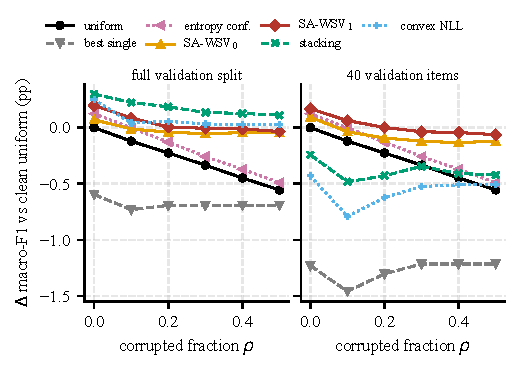
\includegraphics[width=0.84\columnwidth]{fig_stress.pdf}
\caption{Stress test: macro-F1 difference to clean uniform soft voting as one learner's class probabilities are swapped on a fraction $\rho$ of items (mean over corpora, seeds and corrupted learners).}
\label{fig:stress}
\end{figure}

\subsection{The Confidence Term and Calibration}
Within each learner the entropy confidence ranks correct above incorrect predictions (AUROC 0.73 to 0.84), and on contested posts it gives correct learners 0.65 to 0.67 of the weight against 0.60 under uniform weights. Across learners the scales differ, and the term makes the fused posterior over-confident: \rco{} has pooled ECE 0.043, 0.060 and 0.039 against 0.017 to 0.020 for uniform voting and for \rcz. Temperature-scaling the inputs lowers this only on EV-Public (to 0.032) and leaves macro-F1 practically unchanged (equivalent within $\pm0.5$ points on EV-Norm and EV-Public, $\pm1$ on EV-Raw) and the tail heavy (CVaR$_5$ $-0.87$); replacing confidences by within-learner percentiles is worse ($-0.72$ points on EV-Raw).

\subsection{Cross-Corpus Transfer}
Table~\ref{tab:transfer} reports zero-shot transfer. Uniform voting loses 15.3 points on average, from a gain of 2.6 (EV-Public to EV-Twitter) to a loss of 30.9 on EV-YouTube, whose stemmed, stop-word-free text confounds preprocessing with domain and label shift. Positive recall falls by 23.6 points on average, negative recall by 5.5. XLM-R degrades least (13.2 points) and mBERT most (20.1). Errors decorrelate under shift (error correlation 0.55 to 0.47), yet the soft-voting rules of group (i) stay within one point of each other in 8 of 10 directions, \rcz{} changes uniform voting by $+0.07$ points on average, and static weights fitted on the target labels, an oracle, would gain only 0.4 to 2.7 points.

\begin{table}[t]
\caption{Zero-shot transfer: macro-F1 of uniform soft voting on the target (mean over seeds 1--4 and folds); in-domain value in parentheses.}
\label{tab:transfer}
\centering
\footnotesize
\setlength{\tabcolsep}{3pt}
\begin{tabular}{lccccc}
\toprule
Source $\backslash$ target & Norm & Raw & Public & Twitter & YouTube \\
\midrule
EV-Norm   & (89.3) & -- & 74.5 & 80.8 & 60.4 \\
EV-Raw    & -- & (88.3) & 74.9 & 78.7 & 59.8 \\
EV-Public & 76.9 & 72.7 & (85.5) & 88.1 & 54.5 \\
\bottomrule
\end{tabular}
\end{table}

\subsection{Annotation Ambiguity}
The two labelling passes agree on 78.9\% of the 1{,}342 posts labelled in both (Cohen's $\kappa=0.58$, 95\% interval 0.54 to 0.62); 21.1\% were revised, almost symmetrically (141 negative to positive, 142 positive to negative). As the review was not blind, this agreement is likely an upper bound on independent agreement. Errors concentrate on revised posts: within a seed, posts all five learners miss (70 to 83\% revised) are 6.4 to 8.5 (EV-Norm) and 9.5 to 12.7 (EV-Raw) times more likely to have been revised than posts all learners get right; the ensemble is correct on 61 to 67\% of revised posts against 95 to 96\% of the others, and agrees with the first annotator on 33 to 39\% of them. The ensemble's confidence in the final label predicts revision with AUROC 0.86 to 0.89 (0.83 to 0.84 for label-free entropy), and confident learning \cite{northcutt2021} flags 3.8\% of posts, 79 to 84\% of them revised.

\subsection{Computational Cost}
Fine-tuning a learner on a fold takes a median of 18 to 27~s on the primary corpus and 46 to 65~s on EV-Public, 3.4 GPU-hours for all 375 runs. Inference costs about 1~ms per post per learner. Fitting \rc{} takes 14 to 38~ms per fold on one CPU core, almost all of it the bootstrap (Monte Carlo error of $\lambda$: 0.005 at $B=1{,}000$); applying a rule costs under 1\,$\mu$s per post.

\section{Discussion}

\subsection{What the Fusion Rule Can and Cannot Do}
The largest effect is the choice of encoder: mBERT trails every monolingual encoder everywhere, as it trailed IndoBERT on Indonesian sentiment in \cite{rust2021}, who trace such gaps to pre-training data size and tokenizer fit, while XLM-R is competitive on EV-Public and degrades least under shift. With the encoders fixed, the fusion rule matters little, whatever a single seed suggests. The mechanism is low diversity: about two effective voters among five, and seeds add even less, in line with the conjecture that PLM ensembles fine-tuned from one checkpoint are limited by their correlation \cite{xiao2022}. Validation noise is not the main obstacle: the validation split ranks learners on two of the three corpora (Section~\ref{sec:noise}), so the flat comparison is due mostly to correlated errors.

\subsection{\rc{} as a Risk-Control Mechanism}
\rc{} does not reliably raise accuracy, nor does any of the 26 rules here; its value lies in the shape of the outcome distribution. Shrinkage moves the reliability weights toward their $\lambda=0$ limit as far as the paired bootstrap says the spread is noise, so with $\gamma=0$ the rule interpolates between uniform voting, which is safe, and log-odds weighting, which removes a learner no better than chance: it keeps uniform voting's bounded downside on clean pools and the reliability term's protection against a degraded learner, without fitting any parameter. Learned combiners have the best full-split means but a downside an order of magnitude larger at 20 to 80 items, consistent with reports that optimised ensemble weights can overfit limited validation data \cite{purucker2023}. The confidence term is a separate gamble: it raises the mean a little but enlarges the tail and the fused over-confidence, because softmax confidences are on learner-specific scales, and temperature scaling repairs neither the tail nor, on two corpora, the calibration. We therefore recommend $\gamma=0$ when the downside matters; this recommendation is informed by these data and should be confirmed on new corpora.

\subsection{Transfer and Residual Errors}
Corpus shift is the largest practical risk: a model trained on one Indonesian EV corpus can lose up to 31 points on another, and no static weighting recovers much of it, in line with the out-of-distribution decay reported for PLMs \cite{yang2023}. In domain, the remaining errors are largely ambiguous posts: posts every model misses were mostly revised by the second annotator, and ensemble disagreement with the final label identifies revisions well, as annotation-error detection studies report \cite{klie2023}. Inspected examples are questions, adverts or mixed opinions, pointing to label variation \cite{plank2022} and aspect-level schemes \cite{canavara2025, nugroho2024zero} rather than a new voting rule.

\subsection{Limitations}
The corpora are binary and of moderate size, and one hyper-parameter configuration was used. The second labelling pass saw the first, and the public corpora's labelling protocols are undocumented. Validation splits both select checkpoints and fit fusion rules, which makes validation reliabilities optimistic (by 1.4 points). The recommendation of $\gamma=0$ and all risk figures rest on five seeds and three corpora with strongly correlated learners; heterogeneous pools may behave differently.

\subsection{Conclusions}
Across 375 fine-tuning runs and 26 fusion rules for Indonesian EV sentiment, the encoder matters far more than the fusion rule, and no rule beats uniform soft voting reliably, because the learners err together. Shrinking validation reliabilities by a James--Stein factor with a paired-bootstrap noise estimate gives a rule with a bounded downside: in its confidence-free form it gains a little on average, rarely loses, ignores a learner no better than chance, and reduces to uniform voting when the evidence for weighting is noise. Effort is better spent on encoder choice, normalisation, robustness to corpus shift and annotation quality.

\section*{Author Contributions}
{\small B. Juarto led the study, implementation, experiments, analysis, and drafting. K. A. Tiara contributed ideas, literature review, writing, and revision. Both authors approved the manuscript.\par}

\section*{Data Availability}
{\small\raggedright\parindent=1em Analysis code, numerical labels, fold indices, stored posteriors, and aggregate results are available at \texttt{https://github.com/SeedFlora/projectEV}. The primary EV-Norm/EV-Raw text and labelling worksheets are available on request, subject to privacy and redistribution review. EV-Public, EV-Twitter and EV-YouTube originate from \emph{Dataset-Komentar-Kendaraan-Listrik} (ryasakbar060), \emph{analisis-sentimen-kendaraan-listrik} (wynernawati), and \emph{analisis-sentimen-terkait-intensif-mobil-listrik} (billycemerson); original-source links and reproduction instructions are provided in the repository.\par}

\section*{Acknowledgment}
{\small An AI assistant was used for brainstorming and paraphrasing to improve clarity. The authors reviewed and verified all content and take full responsibility for it.\par}

\begin{thebibliography}{00}
\bibitem{saraswati2025} N. W. S. Saraswati, I. W. D. Suryawan, I. D. M. K. Muku, I. K. A. Bisena, and D. A. K. Pramita, ``Indonesian public sentiment toward electric vehicles: Analysis of social media data,'' \emph{Sinkron: Jurnal dan Penelitian Teknik Informatika}, vol. 9, no. 3, pp. 1823--1834, Jul. 2025, doi: 10.33395/sinkron.v9i3.15179.
\bibitem{ekatama2023} R. A. Ekatama, M. Rahardi, A. Aminuddin, and F. F. Abdulloh, ``Sentiment analysis of electric vehicles in Indonesia using support vector machine and na\"{\i}ve Bayes,'' in \emph{Proc. ICON-SONICS}, 2023, pp. 120--125, doi: 10.1109/ICON-SONICS59898.2023.10435277.
\bibitem{devlin2019} J. Devlin, M.-W. Chang, K. Lee, and K. Toutanova, ``BERT: Pre-training of deep bidirectional transformers for language understanding,'' in \emph{Proc. NAACL-HLT}, 2019, pp. 4171--4186, doi: 10.18653/v1/N19-1423.
\bibitem{wilie2020} B. Wilie et al., ``IndoNLU: Benchmark and resources for evaluating Indonesian natural language understanding,'' in \emph{Proc. AACL-IJCNLP}, 2020, pp. 843--857, doi: 10.18653/v1/2020.aacl-main.85.
\bibitem{ganaie2022} M. A. Ganaie, M. Hu, A. K. Malik, M. Tanveer, and P. N. Suganthan, ``Ensemble deep learning: A review,'' \emph{Eng. Appl. Artif. Intell.}, vol. 115, Art. no. 105151, Oct. 2022, doi: 10.1016/j.engappai.2022.105151.
\bibitem{bouthillier2021} X. Bouthillier et al., ``Accounting for variance in machine learning benchmarks,'' in \emph{Proc. MLSys}, vol. 3, 2021, pp. 747--769.
\bibitem{sellam2022} T. Sellam et al., ``The MultiBERTs: BERT reproductions for robustness analysis,'' in \emph{Proc. ICLR}, 2022.
\bibitem{ha2021} S. Ha, D. J. Marchetto, S. Dharur, and O. I. Asensio, ``Topic classification of electric vehicle consumer experiences with transformer-based deep learning,'' \emph{Patterns}, vol. 2, no. 2, Art. no. 100195, Feb. 2021, doi: 10.1016/j.patter.2020.100195.
\bibitem{alhari2022} M. I. Alhari, O. N. Pratiwi, and M. Lubis, ``Sentiment analysis of the public perspective electric cars in Indonesia using support vector machine algorithm,'' in \emph{Proc. ICSINTESA}, 2022, pp. 155--160, doi: 10.1109/ICSINTESA56431.2022.10041604.
\bibitem{wijaya2024} D. R. Wijaya, G. M. A. Sasmita, and W. O. Vihikan, ``Sentiment analysis of Indonesian citizens on electric vehicle using FastText and BERT method,'' \emph{J. Inf. Syst. Informatics}, vol. 6, no. 3, pp. 1360--1372, Sep. 2024, doi: 10.51519/journalisi.v6i3.784.
\bibitem{nugroho2025} M. B. Nugroho, A. K. Zyen, and N. A. Widiastuti, ``Multiclass sentiment analysis of electric vehicle incentive policies using IndoBERT and DeBERTa algorithms,'' \emph{J. Appl. Inform. Comput.}, vol. 9, no. 3, pp. 910--919, Jun. 2025, doi: 10.30871/jaic.v9i3.9511.
\bibitem{canavara2025} G. A. Canavara and H. Irawan, ``Aspect-based sentiment analysis of Indonesian YouTube comments on electric and hybrid vehicles using IndoBERT and IndoRoBERTa,'' in \emph{Proc. ICDSG}, 2025, pp. 43--48, doi: 10.1109/ICDSG67714.2025.11381348.
\bibitem{nugroho2024zero} S. A. Nugroho and S. Widianto, ``Exploring electric vehicle adoption in Indonesia using zero-shot aspect-based sentiment analysis,'' \emph{Sustain. Oper. Comput.}, vol. 5, pp. 191--205, 2024, doi: 10.1016/j.susoc.2024.08.002.
\bibitem{conneau2020} A. Conneau et al., ``Unsupervised cross-lingual representation learning at scale,'' in \emph{Proc. ACL}, 2020, pp. 8440--8451, doi: 10.18653/v1/2020.acl-main.747.
\bibitem{rust2021} P. Rust, J. Pfeiffer, I. Vuli\'{c}, S. Ruder, and I. Gurevych, ``How good is your tokenizer? On the monolingual performance of multilingual language models,'' in \emph{Proc. ACL-IJCNLP}, 2021, pp. 3118--3135, doi: 10.18653/v1/2021.acl-long.243.
\bibitem{seth2023} P. Seth, R. Goel, K. Mathur, and S. Vemulapalli, ``RSM-NLP at BLP-2023 Task 2: Bangla sentiment analysis using weighted and majority voted fine-tuned transformers,'' in \emph{Proc. BLP}, 2023, pp. 305--311, doi: 10.18653/v1/2023.banglalp-1.40.
\bibitem{batra2021} H. Batra, N. S. Punn, S. K. Sonbhadra, and S. Agarwal, ``BERT-based sentiment analysis: A software engineering perspective,'' in \emph{Proc. DEXA}, LNCS, vol. 12923. Cham, Switzerland: Springer, 2021, pp. 138--148, doi: 10.1007/978-3-030-86472-9\_13.
\bibitem{yang2025} S. Yang, J. Xing, Z. Dong, and Z. Liu, ``Heterogeneous ensemble sentiment classification model integrating multi-view features and dynamic weighting,'' \emph{Electronics}, vol. 14, no. 21, Art. no. 4189, Oct. 2025, doi: 10.3390/electronics14214189.
\bibitem{wu2026} X. Wu, H. Ke, and Q. Wu, ``An improved weighted average ensemble method for textual sentiment analysis with Transformer and FNet,'' \emph{Information}, vol. 17, no. 6, Art. no. 605, Jun. 2026, doi: 10.3390/info17060605.
\bibitem{elgabry2026} M. Elgabry and A. Hamdi, ``Confidence-credibility aware weighted ensembles of small LLMs outperform large LLMs in emotion detection,'' in \emph{Proc. IRICT}, LNDECT, vol. 293. Cham, Switzerland: Springer, 2026, pp. 170--179, doi: 10.1007/978-3-032-23035-5\_16.
\bibitem{alkaff2026} M. Alkaff, E. S. Wijaya, F. Fadliyanur, M. Bahit, and S. N. Ilyasa, ``Indonesian hate speech detection under class imbalance using a soft-voting ensemble of IndoBERTweet and IndoRoBERTa,'' \emph{J. RESTI}, vol. 10, no. 3, pp. 814--824, Jun. 2026, doi: 10.29207/resti.v10i3.7681.
\bibitem{purucker2023} L. O. Purucker and J. Beel, ``CMA-ES for post hoc ensembling in AutoML: A great success and salvageable failure,'' in \emph{Proc. AutoML Conf.}, PMLR, vol. 224, 2023, pp. 1--23.
\bibitem{kuncheva2014} L. I. Kuncheva, \emph{Combining Pattern Classifiers: Methods and Algorithms}, 2nd ed. Hoboken, NJ, USA: Wiley, 2014, doi: 10.1002/9781118914564.
\bibitem{efron2021} B. Efron and T. Hastie, \emph{Computer Age Statistical Inference: Algorithms, Evidence, and Data Science}, student ed. Cambridge, U.K.: Cambridge Univ. Press, 2021, doi: 10.1017/9781108914062.
\bibitem{guo2017} C. Guo, G. Pleiss, Y. Sun, and K. Q. Weinberger, ``On calibration of modern neural networks,'' in \emph{Proc. ICML}, 2017, pp. 1321--1330.
\bibitem{xiao2022} Y. Xiao, P. P. Liang, U. Bhatt, W. Neiswanger, R. Salakhutdinov, and L.-P. Morency, ``Uncertainty quantification with pre-trained language models: A large-scale empirical analysis,'' in \emph{Findings EMNLP}, 2022, pp. 7273--7284, doi: 10.18653/v1/2022.findings-emnlp.538.
\bibitem{klie2023} J.-C. Klie, B. Webber, and I. Gurevych, ``Annotation error detection: Analyzing the past and present for a more coherent future,'' \emph{Comput. Linguist.}, vol. 49, no. 1, pp. 157--198, Mar. 2023, doi: 10.1162/coli\_a\_00464.
\bibitem{northcutt2021} C. Northcutt, L. Jiang, and I. Chuang, ``Confident learning: Estimating uncertainty in dataset labels,'' \emph{J. Artif. Intell. Res.}, vol. 70, pp. 1373--1411, Apr. 2021, doi: 10.1613/jair.1.12125.
\bibitem{plank2022} B. Plank, ``The `problem' of human label variation: On ground truth in data, modeling and evaluation,'' in \emph{Proc. EMNLP}, 2022, pp. 10671--10682, doi: 10.18653/v1/2022.emnlp-main.731.
\bibitem{wibowo2021} H. A. Wibowo et al., ``IndoCollex: A testbed for morphological transformation of Indonesian colloquial words,'' in \emph{Findings ACL-IJCNLP}, 2021, pp. 3170--3183, doi: 10.18653/v1/2021.findings-acl.280.
\bibitem{ulmer2022} D. Ulmer et al., ``Experimental standards for deep learning in natural language processing research,'' in \emph{Findings EMNLP}, 2022, pp. 2673--2692, doi: 10.18653/v1/2022.findings-emnlp.196.
\bibitem{mcnemar1947} Q. McNemar, ``Note on the sampling error of the difference between correlated proportions or percentages,'' \emph{Psychometrika}, vol. 12, no. 2, pp. 153--157, Jun. 1947, doi: 10.1007/BF02295996.
\bibitem{yang2023} L. Yang et al., ``GLUE-X: Evaluating natural language understanding models from an out-of-distribution generalization perspective,'' in \emph{Findings ACL}, 2023, pp. 12731--12750, doi: 10.18653/v1/2023.findings-acl.806.
\end{thebibliography}


\end{document}
